% -*- mode: latex; mode: auto-fill; coding: utf-8; -*-

Physics is a science based on experiments where phenomena of nature
are observed with the objective of finding patterns and
principles. These patterns and principles are called theories or, when
they are commonly accepted, \defit{laws of physics}
\citebook{page~1}{book:uni-physics}.
%
As already touched upon in section \vref{sec:simulator}, the
simulator incorporates such physical laws to simulate
deformation and fragmentation of solid material. This
chapter introduces the physical theories needed to create a
 simulation model.
%
The aim is to assemble a theoretical model for deformation and
fragmentation based on the laws observed and generally accepted by
physicists.
%
Note that the physical laws used are idealized models, meaning
that the models are simplified versions of real phenomena and that
concepts of little importance for the overall result are neglected
\citebook{page~3}{book:uni-physics}.
%
In this respect we do not model material at the level of particles
as the effects of individual particles are not detectable when
larger volumes of matter are considered. This is called large-scale
mechanics in contrast to quantum mechanics, which deals with laws at
the level of atoms. Large-scale mechanics is valid when the size of
the material analysed is much larger than the size of an atom
\citebook{page~1}{book:continuum-mechanics}. \\

%A part of physics, \defit{mechanics}, are of special interest.
The subgroups of special interest are \defit{statics},
\defit{dynamics} and \defit{continuum mechanics}.
%
As the theory of continuum mechanics is quite complex, we will start
off gently by revisiting basic university physics in the context of
statics and dynamics. Here we define various physical quantities,
their corresponding units and how they are related.

% To get a visual image of the quantities, we need to set the
% scene \{tic}{we need to identify what needs to be modelled?}. 
% So what needs to be modeled? The basic idea is to manipulate an object
% through \defit{forces}. The object should react
% realistically and naturally to these forces. This object can be made of
% different material and have diverse shapes.\{tic}{The object
%   material and shape can vary.}

\section{Statics and Dynamics}
In statics, we only analyse objects that do not move. This enables
us to describe and relate various phenomena acting upon an object.
%
The next step is dynamics, where objects are allowed to move
but not to deform. Dynamics expands the analytical
method by allowing movement and rotation.
%
In statics an object is viewed as a single point which describes its
position. In dynamics objects are modeled by their position and
orientation. Statics and dynamics make these assumptions so objects
are less complex to analyse. In continuum mechanics objects are
represented by volumetric elements, which are more complex.

%define: space, time and reference frame
\subsection{Space and Time}
Within statics and dynamics, objects and forces alone are not enough
when analysing a physical system. The concept of an object at
rest or in motion requires a \defit{frame of reference}. A frame of
reference is any kind of coordinate system which enables us to uniquely
define the position of a body in three-dimensional space. To
describe motion the frame of reference must be fixed so only motion of
the moving body is considered.
%
By introducing time we can refer to an object at a given
time, hereby describing the object's \defit{velocity}
and \defit{acceleration}.
%
Complying with the SI system for units, distance is measured in meters
($m$), time in seconds ($s$), velocity in $m/s$, and acceleration in
$m/s^2$.

%interne vs externe forces, body and surface forces (static p. 78-80).
\subsection{Forces}
In mechanics there are many different types of forces,
therefore we need some basic terms to describe them. A force has a
direction and a magnitude. The direction is referred to as the
\defit{line of action}. The magnitude determines the size of the
force and is measured in newton ($N$). A force acts upon an object at
a specific point as illustrated in figure
\vref{fig:gravitationalforce}: A force is depicted in a
\defit{free-body diagram} as an arrow mounted at the point in which it
acts.

\begin{figure}
  \centering
  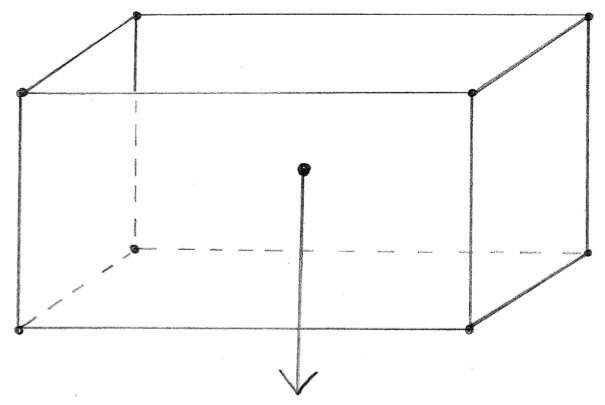
\includegraphics[width=6cm]{./images/physics_gravitationalforce.png}
\caption{Free-body diagram of the gravitational force acting upon a box.}
\label{fig:gravitationalforce}
\end{figure}

In mechanics an object is composed of two distinct concepts: a
\defit{surface} and a \defit{body} (note that the entire object is
often referred to as the body, which can be a little confusing).
%
Forces can be divided into different types, the types used in this
thesis are: body contra surface and internal contra external.
%
External forces act upon a physical system from the outside and can
not be generated by the system itself. 
%
An example of an external body force is the gravitational force as
illustrated in figure \vref{fig:gravitationalforce}. 
When two objects collide, a contact force occurs between
the colliding surfaces. This is an example of an external surface
force, and is illustrated in figure \vref{fig:contactforce}.
%
Internal forces do not occur in statics and dynamics because the
various internal parts of an object cannot move and hereby
interact. When modelling deformations, various parts of an object
can interact, hence we need internal forces.
In section \vref{sec:internal-forces} internal
forces will be introduced.

\layoutnewpage

% \begin{figure}
%   \centering
%   \includegraphics[width=6cm]{./images/physics_contactforce.png}
% \caption{A contact force.}
% \label{fig:contactforce}
% \end{figure}

\begin{figure}
  \centering
  \subfloat[]{
    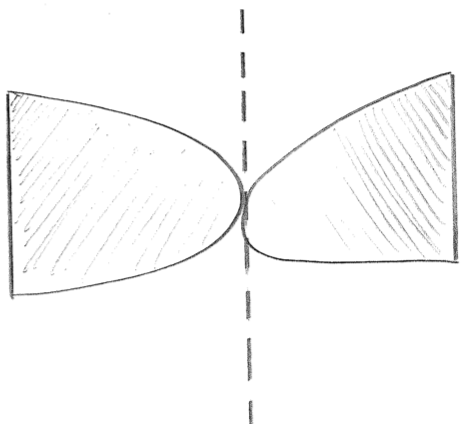
\includegraphics[width=6cm]{./images/physics_contactforce_a.png}
    %\label{fig:worka}
  }
  \subfloat[]{
    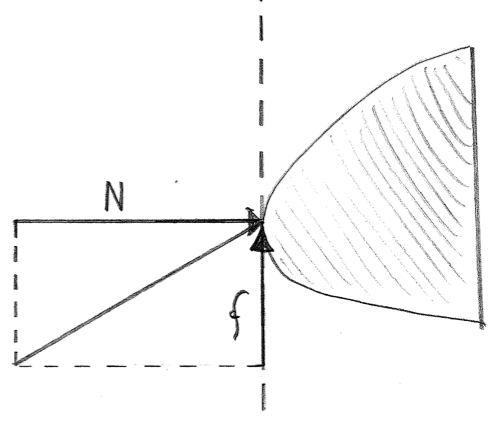
\includegraphics[width=6cm]{./images/physics_contactforce_b.png}
    %\label{fig:workb}
  }
  \caption{A contact force.}
  \label{fig:contactforce}
\end{figure}

Forces can be represented by vectors and therefore be resolved into
components. Resolving a force into its components sometimes eases the
analysis of a problem. Figure \vref{fig:contactforce} illustrates the contact force
resolved into two components $N$ and $f$, defined as the force normal
to the contact plane and a friction force along this plane,
respectively \citebook{page~80}{book:static-mechanics}.

\subsection{Equilibrium}
\label{sec:equilibrium}
To analyse a problem in physics, for example a free-body diagram,
the notion of equilibrium is used.
%
Equilibrium in general means an unchanging state or a state of
balance. In mechanics \defit{equilibrium} is defined as:

\begin{definition}
\label{def:equilibrium}
A body is in equilibrium if it is either at rest or moving in a
straight line with constant velocity \citebook{page~97}{book:uni-physics}.
\end{definition}

If a body is in equilibrium we can use definition
\vref{def:equilibrium} to analyse entities influencing the object's
behavior.
%
Depending on what types of problems we consider and which kind of
results we are seeking, this definition of equilibrium must be
interpreted differently to meet the constraints imposed on a given
problem.
%
We now consider three interpretations of the definition, with
increasing generality of the problems they capture, in each step
lowering the number of constraints imposed on the problem. \\

% equilibrium (static p. 205 and 273)
\subsubsection{Equilibrium for Fixed Objects}
\label{sec:equilibrium_for_fixed_objects}
When more than one external force act upon an object, the forces can
be added to yield the \defit{sum of forces}. The sum of forces is the
effective net force acting upon the body. We use this knowledge to
establish equilibrium for fixed objects.
%The sum of forces is calculated by: $\sum f = f_1 + f_2 + ... + f_n$.
Statics define equilibrium as \defit{conservation of forces} defined by:

\begin{definition}
\label{static-equilibrium}
A body that can be modeled as a particle is in equilibrium whenever
the vector sum of the forces acting on it is zero.
That is: $\sum f = 0$
\citebook{page~329}{book:uni-physics}.
\end{definition}

We can use this definition of equilibrium to analyse problems involving
fixed objects. That is: We can calculate unknown forces. Imagine that
we apply external gravitational force to an object placed on a
table. With the equilibrium equation we can calculate the force
provided by the table to support the object. \\

\subsubsection{Equilibrium for Moving Objects}
Equilibrium for fixed objects does not apply to moving bodies. In order
to model motion, more theory is needed. The simplest moving body is a rigid
body. A rigid body is allowed to move but not to deform. 
Movement has two distinct components: \defit{translation} and
\defit{rotation}. When applying the theory of equilibrium on rigid
bodies, translation and rotation must be included into the definition
of equilibrium.

\begin{definition}
\label{dynamic-equilibrium}
In addition to the requirements of equilibrium for fixed objects, the
sum of all torques due to all external forces acting on the body, with
respect to any specified point, must be zero.
That is: $\sum f = 0 \wedge \sum m = 0$
\citebook{page~329-330}{book:uni-physics}.
\end{definition}

\defit{Torque} or \defit{angular momentum} is a measure of a
rotational force. Torque is defined as: $m = r \times f$, where the force
$f$ is acting on a line of action perpendicular to the \defit{lever arm}, in
a distance of $r$ \citebook{page~294-296}{book:uni-physics}. Note that
equilibrium for fixed objects is a subset of equilibrium for moving
objects, and is exactly the special case where all torques are zero. \\

% \subsubsection{Equilibrium for Deformable Objects}
% Even with equilibrium for moving objects we do not capture the entire
% problem. As we want to model deformations we need to introduce
% continuum mechanics.
% In continuum mechanics we can no longer view the body as a single
% point, instead infinitesimal calculus is used for analysing the body.
% %
% To enable equilibrium analysis of a continuum we introduce the more
% general definition: \defit{mechanical equilibrium}. This definition is
% an alternative definition of equilibrium which can be apply to
% \defit{conservative} systems, and used in collaboration with
% infinitesimal calculus and continuum mechanics:
% %
% \begin{definition}
% \label{mechanical-equilibrium}
% An object is in mechanical equilibrium if the forces that do work as
% the result of a virtual displacement are conservative, i.e. the change in
% the total potential energy is zero: $\delta \Delta E_U = 0$
% \citebook{page~573}{book:static-mechanics}.

% %A system is in mechanical equilibrium if its position in configuration
% %space is a point at which the gradient of the potential energy is zero.
% %\citebook{page~?}{}
% %http://www.economicexpert.com/a/Mechanical:equilibrium.html
% %***gradient of the potential energy = forces, uni-physics, p. 215

% \end{definition}

% To understand this abstract definition, we introduce the terms:
% \defit{work}, \defit{energy} and means of \defit{conservation}. We
% also need to define what means \defit{virtual}, in context of
% mechanics. Again we note, although this time not directly apparent,
% that equilibrium for moving objects is a subset of mechanical
% equilibrium. The theory of continuum mechanics is further elaborated
% in section(\vref{sec:continuum}).


\subsubsection{Equilibrium for Deformable Objects}
\label{sec:equilibrium-for-deobj}
When considering deformable objects, we no longer use forces as
the quantity to define equilibrium.
%
% \{To explain why, we consider the following. 
% When a body is deformed by external forces the
% internals of the body are stretched or compressed generating internal
% forces. The external forces acting upon the body can in opposite
% directions. If the forces are of the same
% magnitude and in opposite directions then their sum  will be zero.
% Clearly this is not enough information for the body to bounce back,
% when the external forces are released. To record enough
%   information both the distance and direction in which the forces
%   stretch or compress the body must be taken into account.}
%
To define equilibrium for a deformable object, we will instead used
the \defit{principle of conservation of energy} as defined in
definition \vref{def:pmpe}.
 
\begin{definition}
\label{def:pmpe}
The mechanical energy in a conservative system is always constant
\citebook{page~160}{book:dynamic-mechanics}.
\end{definition}

In order to understand definition \vref{def:pmpe} we need to
introduce: work, kinetic energy, conservative systems, potential
energy, and mechanical energy. Again we note, although this time not
directly apparent, that equilibrium for moving objects is a subset of
equilibrium for deformable objects. In section \vref{sec:continuum},
when the theory of continuum mechanics is elaborated, we will return
to what equilibrium is for a deformable object, in that section it will be
applied to a continuum.

\subsection{Work}
\label{sec:work}
% enhed N*m = J, uniphysics p. 165
\defit{Work} is the amount of energy transferred by a force acting over a
distance. For a moving body where forces are not uniformly distributed
work is defined in terms of \defit{differential work}. So to calculate
the total work $W$ we
integrate $dW$, where $dW$ is the differential work done by $f$ as a
result of the displacement $dr$. Work is measured in Newton meter
($Nm$) or Joule ($J$) \citebook{page~174-179}{book:uni-physics}.

\begin{equation}
  dW = f \cdot dr = (|f|cos \phi)|dr|
  \qquad \Leftrightarrow \qquad
  W = \int dW = \int f \cdot dr
\end{equation}

Consider a force $f$ acting on an object at point $P$ as illustrated
in figure \vref{fig:worka}. Suppose the object undergoes an infinitesimal
motion, so $P$ is displaced by vector $dr$ (see figure
\vref{fig:workb}). The differential work $dW$ done by $f$ as a result
of the displacement $dr$ can then be illustrated as in figure
\vref{fig:workc}. In this figure the force $f$ is not parallel to $dr$
and therefore only a part of the force produces work. The precise
amount of work produced by $f$ is equal to the length of $f$ projected
onto $dr$ \citebook{page~558}{book:static-mechanics}.

% \begin{figure}
%   \begin{minipage}[b]{0.3\linewidth}
%     \centering
%     \subfloat[]{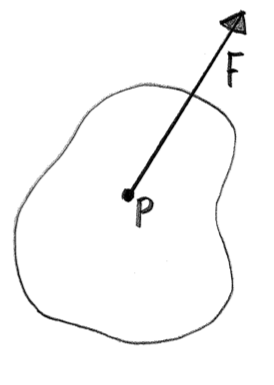
\includegraphics[width=40mm]{./images/physics_work_a.png}}
%   \end{minipage}
%   %\hspace{0.5cm}
%   \begin{minipage}[b]{0.3\linewidth}
%     \centering
%     \subfloat[]{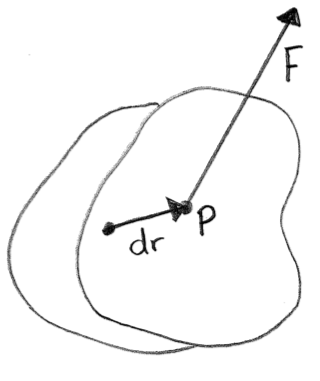
\includegraphics[width=40mm]{./images/physics_work_b.png}}
%   \end{minipage}
%   %\hspace{0.5cm}
%   \begin{minipage}[b]{0.3\linewidth}
%     \centering
%     \subfloat[]{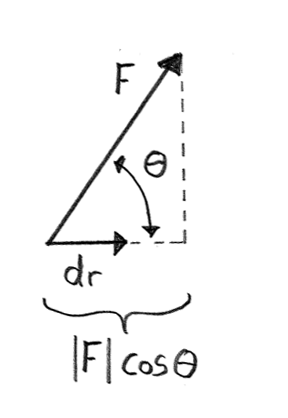
\includegraphics[width=40mm]{./images/physics_work_c.png}}
%   \end{minipage}
% \end{figure}
  
\begin{figure}
  \centering
  \subfloat[A force $f$ acting on an object]{
    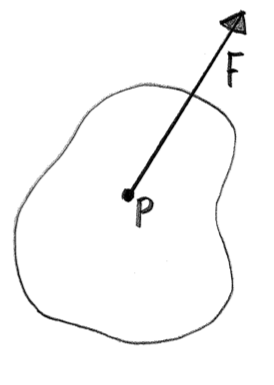
\includegraphics[width=4cm]{./images/physics_work_a.png}
    \label{fig:worka}
  }
  \subfloat[A displacement $dr$ of $P$]{
    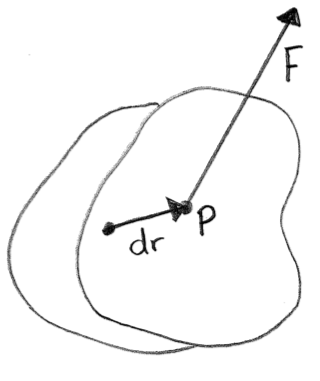
\includegraphics[width=4.5cm]{./images/physics_work_b.png}
    \label{fig:workb}
  }
  \subfloat[$dW=(|f|cos \phi)|dr|$]{
    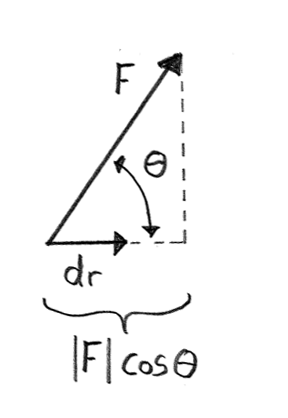
\includegraphics[width=4.3cm]{./images/physics_work_c.png}
    \label{fig:workc}
  }
  \caption{Illustration of work.}
  \label{fig:work}
\end{figure}


% \subsubsection{Virtual Displacement and Virtual Work}
% \label{sec:virtual-work}
% When using the term \defit{virtual} in the context of physics, it
% refers to an imagined scenario. For example: We can talk about a virtual
% displacement of an object event though the object cannot move. The
% virtual displacement is not applied to the object but we can use
% this imaginary displacement to do calculations on the object. In
% mathematical notation virtual is denoted $\delta$. Virtual
% displacement is denoted $\delta r$.
% %
% Virtual work is defined in terms of virtual displacement, and is
% therefore also an imaginary thing.

% \begin{equation}
% \delta W = f \cdot \delta r
% \end{equation}

% Virtual work is used to analyse complete structures via the
% conservation law: \defit{principle of virtual work} to be introduced
% in section \vref{sec:principle-of-virtual-work}
% \citebook{page~558-561}{book:static-mechanics}.

\subsection{Energy}
% enhed J
Although work and \defit{energy} are related and both are measured in
Joule (J), they are not entirely equal concepts. Work refers to a force
acting over a distance. Energy on the other hand is
used when referring to the amount stored or produced by an
object. We use two concepts to describe an object's energy: \defit{Kinetic
  energy} and \defit{potential energy}. 

\subsubsection{Kinetic Energy}
\defit{Kinetic energy} is the energy of motion. Whenever an object moves it
possesses kinetic energy. The amount of kinetic energy within an object
with mass $m$ and velocity $v$ is defined as the work needed to
accelerate the mass $m$ from rest to velocity $v$. The object maintains
its kinetic energy as long as the velocity is constant. If the
velocity increases or decreases so does the kinetic energy. It would
require the same amount of work to decelerate an object to rest, as it
took to accelerate it to velocity $v$. The force required to
decelerate the object has to be in the opposite
direction. The kinetic energy $E_K$ of an object is defined by
\citebook{page~164-165}{book:uni-physics}:

\begin{equation}
E_K = \frac{1}{2} m v^2
\end{equation}

Kinetic energy is related to work by the \defit{work-energy theorem},
which states that work equals the change in kinetic energy
\citebook{page~170}{book:uni-physics}:

\begin{equation}
W = E_K^1 - E_K^0 = \Delta E_K
\end{equation}

\subsubsection{Potential Energy}
\defit{Potential energy}, denoted $E_U$, is the energy stored within a
physical system. An
object can possess potential energy as a result of its position. If for
example a heavy weight is elevated and held above the ground it
possesses potential energy. The energy stored has the potential to be
converted into a different form of energy, e.g. kinetic
energy. Compressing a spring is another way of storing potential
energy within an object. If the force compressing the spring is
removed the spring's restoring force will make it return to its
original position. Potential energy exists when an object 
is displaced and there are forces acting towards bringing
the object back to its original position. 
%

\subsubsection{Conservative and Non-conservative Systems}
When kinetic energy can be converted to potential energy, and back
again, we say that there is a two-way conversion of energy. Systems
with the two-way conversion property are \defit{conservative systems},
those without are \defit{non-conservative systems}. A system where
energy is turned into heat is an example of the latter
\citebook{page~209-210}{book:uni-physics}.
Conservative systems are isolated and have the property that energy
does not dissipate.

\subsubsection{Conservation of Mechanical Energy}
\label{sec:conser-of-me}
When dealing with a conservative system the total amount of
energy is referred to as the mechanical energy ($E_M$), and is defined
by:

\begin{equation}
\label{eq:mech-energy}
E_M = E_K + E_U
\end{equation}

In a conservative system no energy dissipates therefore the mechanical
energy within the system is constant.
Kinetic energy can be stored by converting it to potential energy. The
classic example is: When throwing a ball upwards, kinetic energy is
converted into potential energy on the way up. On the way down the
opposite happens. The relation that makes this possible is called 
\defit{conservation of mechanical energy} and is a direct consequence
of equation \eqref{eq:mech-energy} for a conservative system
\citebook{page~196}{book:uni-physics}:
%
If we consider an object that is deformed, it has an initial state
(state 0), and a deformed state (state 1). In both states the energy
can be calculated as:

\begin{equation}
E_M^0 = E_K^0 + E_U^0 \qquad E_M^1 = E_K^1 + E_U^1
\end{equation}

if the system is conservative, we know that:

\begin{equation}
\label{eq:external_work_equals_internal_energy}
\begin{aligned}
E_M^0 &= E_M^1  \qquad \Leftrightarrow \\
E_K^0 + E_U^0 &= E_K^1 + E_U^1 \qquad \Leftrightarrow \\
E_K^0 - E_K^1 &= E_U^1 - E_U^0  \qquad \Leftrightarrow \\
- (E_K^1 - E_K^0) &= E_U^1 - E_U^0  \qquad \Leftrightarrow \\
- W &= E_U^1 - E_U^0  \qquad \Leftrightarrow \\
- W &= \Delta E_U
\end{aligned}
\end{equation}

by setting the initial potential energy
$E_U^0$ to zero, we obtain:

\begin{equation}
\label{eq:EW}
E_U^1 = -W 
\end{equation}

% \subsubsection{Principle of Virtual Work for Conservative Forces}
% \label{sec:principle-of-virtual-work}
% Work done by a conservative force can be expressed in terms of its
% potential energy. It can be expressed by using the definition of
% mechanical equilibrium as defined in definition
% \vref{mechanical-equilibrium}.
% %
% The definition states that change in total virtual potential energy is
% zero: $\delta \Delta E_U = 0$.
% %
% And because the mechanical energy $E_M = E_K + E_U = 0$, we know that
% $E_U=-E_K$. So the change in potential energy must be the negative
% change of kinetic energy: $\Delta E_U = - \Delta E_K$. As $\Delta
% E_K = W$, we have that $\delta \Delta E_U = - \delta W = 0$.
% %
% In effect this means that the total virtual work must be zero. That
% is, the work done by the internal forces plus the work done by the external
% forces must be zero, so adding up the work done by the internal forces
% with the work done by the external forces this becomes the
% \defit{principle of virtual work}:

% \begin{equation}
% \label{eq:principle_of_virtual_work}
%   \mbox{total virtual work} = \mbox{internal virtual work} +
%   \mbox{external virtual work} = 0
% \end{equation}
% \begin{equation}
%   \mbox{internal virtual work} = - \mbox{external virtual work}
% \end{equation}

% The principle of virtual work has an important property, it can be
% applied to entire structures. This means that structures composed of
% elements can be analysed \citebook{page~560-561}{book:static-mechanics}.
% A continuum consists of infinitesimal
% elements, therefore the principle of virtual work applies when
% analysing continuums.


\section{Continuum Mechanics}
\label{sec:continuum}
In continuum mechanics we assume that the substance of a body is a
continuously distributed matter, that is distributed
throughout and completely fills the space it occupies. We also assume
that the substance is \defit{homogeneous}, that is, the entire body
consists of the same material. Continuum
mechanics ignores the fact that matter is not continuous at the level
of atoms. By ignoring this we can approximate physical quantities, 
such as energy and work, at the infinitesimal limit.

\subsection{Continuum}
Continuum as a concept describes a material as a fixed region of
space. This region forms the geometrical state of a body. We imagine the
region completely covered by a set of infinitesimal volumetric
elements, called \defit{particles}. The position of all particles at a
time $t$ is called a \defit{configuration}.
%
A particular configuration is chosen as the \defit{reference
  configuration} and each particle in the reference configuration is
identified by the position vector $X$. The reference configuration is often
chosen as the configuration at time $t=0$, where the body
is in an undeformed state and at rest
\citebook{page~4}{book:continuum-mechanics}.

%\layoutpb

\begin{figure}
  \centering
  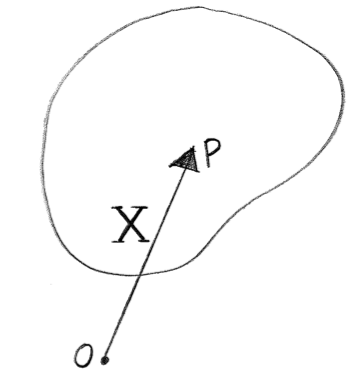
\includegraphics[width=4.5cm]{./images/physics_continuum_body.png}
\caption{A continuum body.}
\label{fig:continuum}
\end{figure}

% \begin{figure}
%   \centering
%   \includegraphics[width=6cm]{./images/wiki-Continuum_body.png}
% \caption{A continuum body}
% \label{fig:continuum}
% \end{figure}

The components of $X$ in the chosen reference frame are referred to as
the \defit{material coordinates}. We say that the particle $P$ occupies
the place $X$ as illustrated in figure \vref{fig:continuum}. Suppose
that the region covered by the body at
\defit{reference time} $t=0$ is $R_0$. If the body moves and at
time $t$ occupies $R$, then we describe this configuration in
relation to the reference configuration by \defit{spatial coordinates}
$x$. 
This scenario is illustrated in figure \vref{fig:displacement}.
The spatial coordinates are the material coordinates plus a
displacement: $x = X + u$, where $u$ is referred to as the
\defit{displacement vector}.
Spatial coordinates can also be calculated as a function $f$ of the
reference configuration and time: $x = f(X,t)$ 
\citebook{page~33-35}{book:continuum-mechanics-anthony}.
Note that by the definition of material and spatial coordinates,
there has to be a one-to-one correspondence between \defit{material
  points} and \defit{spatial points}.

\begin{figure}
  \centering
  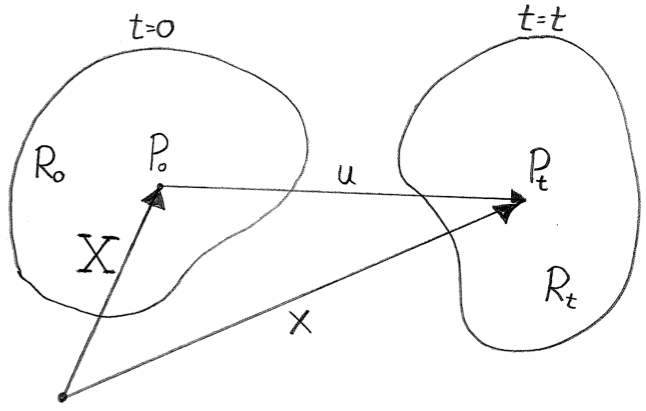
\includegraphics[width=8cm]{./images/physics_displacement.png}
\caption{Displacement of a continuum.}
\label{fig:displacement}
\end{figure}

% \begin{figure}
%   \centering
%   \includegraphics[width=12cm]{./images/wiki-Displacement_of_a_continuum.png}
% \caption{A displacement}
% \label{fig:displacement}
% \end{figure}

\subsection{Deformation}
\label{sec:deformation}
If two configurations of a body are not the same,
one or more of the particles have been displaced. A
\defit{displacement} can be divided into two distinct components: a
\defit{rigid body displacement} and a \defit{deformation}.
%
The difference being whether or not particles have moved in
relation to each other. In a rigid body displacement the relative
inter-particle distances are preserved. In a deformation they are not.

% \begin{figure}
%   \centering
%   \includegraphics[width=8cm]{./images/solid-mechanics-c2-1.png}
% \caption{A deformation}
% \label{fig:deformation}
% \end{figure}

\begin{figure}
  \centering
  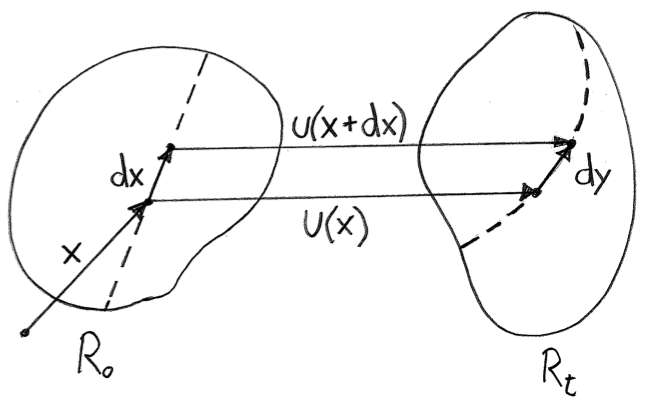
\includegraphics[width=8cm]{./images/physics_deformation_of_line.png}
\caption{Deformation of an infinitesimal line segment.}
\label{fig:deformation_of_line}
\end{figure}

Consider the straight line through the undeformed configuration $R_0$ as
illustrated in figure \vref{fig:deformation_of_line}. After the body
has undergone a deformation the straight line has been mapped to a
smooth curve as illustrated in the deformed configuration $R_t$. Somehow we
would like to represent the line or fiber deformation that takes
place. Focus attention on the line segment $dx$ and imagine that the
length of the line segment is much shorter than the radius of
curvature. The small line segment is straight in the undeformed
configuration and very close to straight in the deformed
configuration. By decreasing the length of the line segments we
improve the approximation of the curvature. This way we can describe
even complex deformations of a body since it is reasonable to neglect
curved material fibers as long as we only consider infinitesimal line
segments. The infinitesimal line segments $dx$ and $dy$ are related by
the ratio: $\frac{dy}{dx}$
\citebook{section~2.1.2}{book:solid-mechanics}.
% the following is directly copied from book:s% olid-mechanics
% \{ To illustrate deformation, imagine drawing a straight line on the
% undeformed configuration as shown in figure
% \vref{fig:deformation-of-line}. The line would be mapped to a smooth
% curve in the deformed configuration. However suppose we focus
% attention on a line segment $dx$, much shorter than the radius of the
% curvature of this curve. The segment would be straight in
% the undeformed configuration, and would also be (almost) straight in
% the deformed configuration. Thus, no matter how complex a deformation
% we impose on a body, infinitesimal line segments are merely
% stretched and rotated by a deformation. The infinitesimal line segments
% $dx$ and $dy$ are related by the ratio: $\frac{dy}{dx}$
% \citebook{section~2.1.2}{book:solid-mechanics}.}
% % the above is directly copied from book:solid
%-machanics
If this ratio is $1$ the material is undeformed, between $0$ and
$1$ it is compressed and if above $1$ it is stretched.
%The concept of stretch and compression
%is illustrated in figure \vref{fig:tension}.
%

% \begin{figure}
%   \centering
%   \subfloat[Stretching]{
%     \includegraphics[width=6cm]{./images/uni-physics-p338-f11-9.png}
%     \label{fig:stretching}
%   }
%   \subfloat[Compression]{
%     \includegraphics[width=6cm]{./images/uni-physics-p339-f11-11.png}
%     \label{fig:compression}
%   }
%   \caption{Stretching contra compression}
%   \label{fig:tension}
% \end{figure}

\subsection{Strain}
\label{sec:physics_strain}
%
Strain is a measure of deformation. Strain represents the amount of
stretch or compression by the relative distance between two particles
in the material body. It is a dimensionless quantity, which can be
expressed as a decimal fraction, or a percentage.
%
In comparison with the ratio $\frac{dy}{dx}$ from section
\vref{sec:deformation}: A strain measure of zero means no deformation,
below or above represents compression or stretching respectively.
%
Strain can be decomposed into \defit{normal strain} and
\defit{shearing strain}.

%To better understand strain, we can divide it into two distinct
%components: Normal or tensile strain and shearing strain.

\subsubsection{Normal Strain}
Normal strain occurs when forces acting parallel to the axes of the
reference frame pull equally throughout the body. Normal strain has
the property of scaling the body in the axial directions. Figure
\vref{fig:normalstrain} illustrates normal strain in one
dimension. Here two external forces pull in opposite
directions on a body hereby stretching it.

\begin{figure}
  \centering
  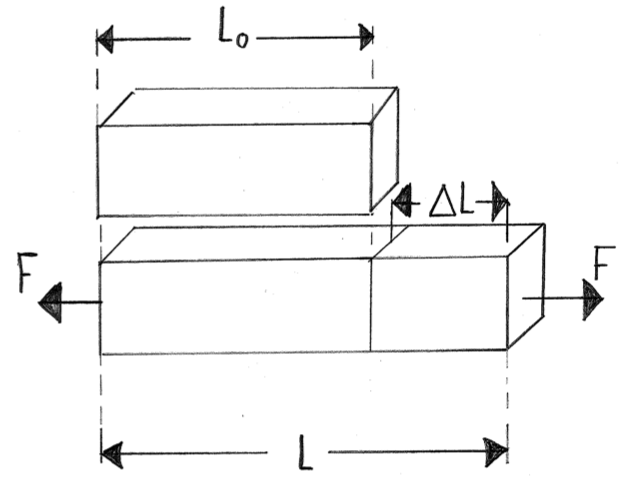
\includegraphics[width=6cm]{./images/physics_normalstrain.png}
\caption{Normal strain.}
\label{fig:normalstrain}
\end{figure}

For the simple case of a body axially loaded,
the normal strain will be uniformly distributed throughout the body
and can be obtained by dividing the displacement (how much the body is
stretched) by the initial length of the body.
%Normal strain is defined to be the displacement (how much the body
%is stretched) divided by the length of the body.

\begin{equation}
\mbox{normal strain: } \frac{l-l_0}{l_0} = \frac{\Delta l}{l_0}
\end{equation}

In general strain is not distributed uniformly over the entire
body, therefore we define strain at a specific point within the
body. Because continuum mechanics assumes strain to be continuous,
differential calculus is used to define strain at any point.
In three dimensions, we have a normal strain component
for each direction in the reference frame. Written out as individual
components this becomes: \citebook{page~659}{book:fem-engineers}

\begin{equation}
\label{eq:individual-normal-strain}
\varepsilon_x = \frac{\partial u_x}{\partial x} \hspace{10 mm}
\varepsilon_y = \frac{\partial u_y}{\partial y} \hspace{10 mm}
\varepsilon_z = \frac{\partial u_z}{\partial z}
\end{equation}

were $u$ is the displacement vector with components $u_x$, $u_y$ and
$u_z$ being the displacement along the $x$, $y$ and $z$ axis of the
reference frame, respectively. Normal strain can be represented on
vector form as:
$\varepsilon = [ \varepsilon_x, \ \varepsilon_y, \ \varepsilon_z ]^T$.

\subsubsection{Shearing Strain}
Shearing strain occurs when the forces are not aligned with the axes
of the reference frame or if they are not uniformly distributed over
the body. This results in distortion of the body's shape as
illustrated in figure \vref{fig:shear-strain}.

% \begin{figure}
%   \centering
%   %\includegraphics[width=6cm]{./images/uni-physics-p343-f11-17.png}
%   \includegraphics[width=14cm]{./images/deformation-shearing-strain.png}
% \caption{Shear strain}
% \label{fig:shearstrain}
% \end{figure}

\begin{figure}
  \centering
  \subfloat[Shearing strain in one direction.]{
    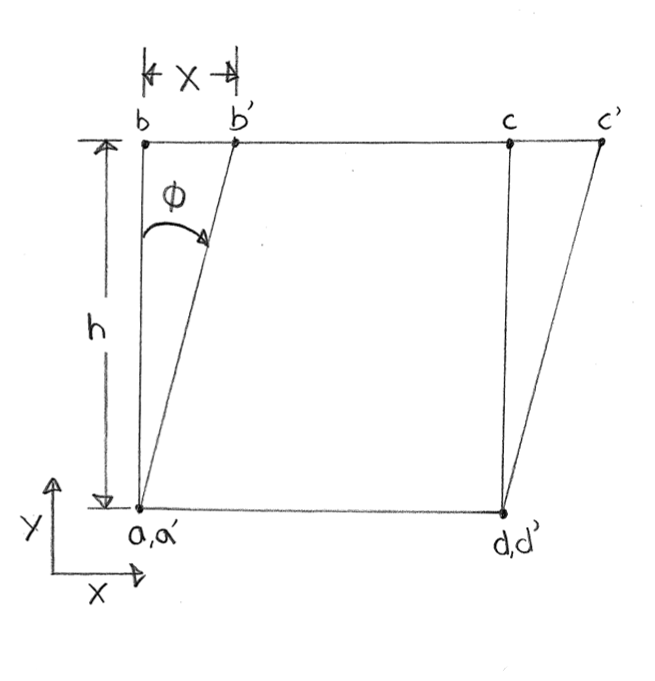
\includegraphics[width=7cm]{./images/physics_shearing_strain_a.png}
    \label{fig:shearing-strain-one-direction}
  }
  \subfloat[Shearing strain in two directions.]{
    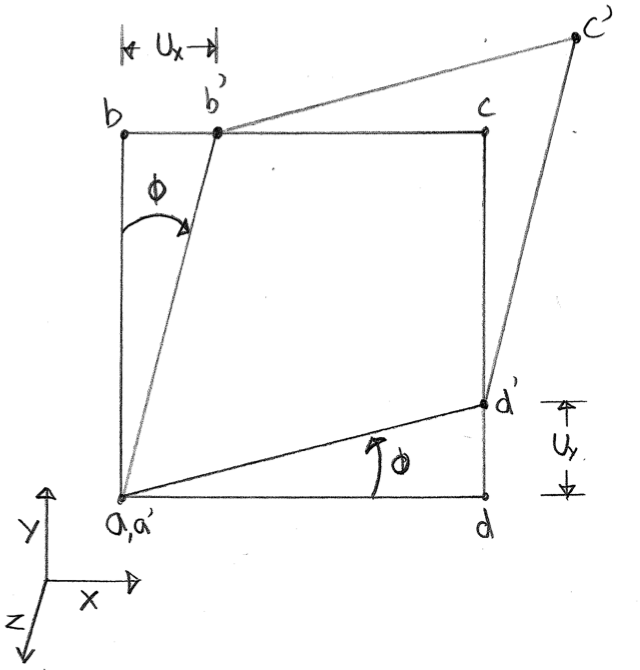
\includegraphics[width=7cm]{./images/physics_shearing_strain_b.png}
    \label{fig:shearing-strain-two-directions}
  }
  \caption{Shearing strain.}
  \label{fig:shear-strain}
\end{figure}

Shear strain is defined as the ratio of the displacement $x$ of the corner
$b$ to the transverse dimension $h$ \citebook{page~343}{book:uni-physics}:

\begin{equation}
\mbox{shear strain: } \frac{x}{h} = tan \phi
\end{equation}

Figure \vref{fig:shearing-strain-one-direction} illustrates basic
shearing strain in one direction. In three dimensions we are
interested in defining the resulting shear strain between
planes. Figure \vref{fig:shearing-strain-two-directions} illustrates
the distortion from shear strain in two directions. To measure the
resulting shear strain between the $xz$-plane and the $yz$-plane the
two individual shearing strains are added.
%
The individual components of the shearing strain in three dimensions are
\citebook{page~7}{book:theory-of-elasticity}:

\begin{equation}
\label{eq:individual-shear-strain}
  \gamma_{xy} = \frac{\partial u_x}{\partial y} +
  \frac{\partial u_y}{\partial x} \hspace{10 mm}
  \gamma_{xz} = \frac{\partial u_x}{\partial z} +
  \frac{\partial u_z}{\partial x} \hspace{10 mm}
  \gamma_{yz} = \frac{\partial u_y}{\partial z} +
  \frac{\partial u_z}{\partial y}
\end{equation}

where $u_x$, $u_y$ and $u_z$ are the axial displacements along the $x$, $y$
and $z$ axis, respectively. Shearing strain can be represented on vector
form as: $\gamma = [ \gamma_{xy}, \ \gamma_{xz}, \ \gamma_{yz} ]^T$.\\

% Applying shear strains along two axes is the same as applying the
% total shear strain along one axis when only measuring the total amount
% of shearing in the given plane. 
% The two distorted squares illustrated in figure \vref{fig:shear-strain}
% are equivalent; the only difference is that the one to 
% the right is translated and rotated slightly.
% Since we are only interested in measuring the resulting shear in each
% plane, and not interested in the resulting orientation of the square,
% we add the two axial shear strains together to obtain
% the equations \eqref{eq:individual-shear-strain}.

%$\frac{\partial u_x}{\partial y}$ represents
%the shear strain in the $x$ direction and $\frac{\partial
%  u_y}{\partial x}$ is in the $y$ direction. 


%internal forces (static p. 448)
\subsection{Internal Forces}
\label{sec:internal-forces}
Internal forces only exist inside an object, where one part of an
object is subjected to forces by another part of the same object
\citebook{page~79}{book:static-mechanics}. 
Internal forces can be experienced simply by stretching a rubber
band. When stretching a rubber band the external force, responsible for
the stretching, induces internal forces. When the external force is
released the rubber band returns to its original shape
hereby releasing the internal forces as well. The way a body behaves
depends on its material properties. How different materials behave is
elaborated in section \vref{mechanical-properties}, but first stress
is introduced as this is a representation of the internal forces.

\subsection{Stress}
\label{sec:physics_stress}
Stress is a measure of the average amount of force exerted per unit
area ($N$/$m^2$). It is a measure of the intensity of the total
internal forces acting within a body across imaginary internal
surfaces, as a reaction to externally applied forces.
%In
%general, stress is expressed as a force $f$ acting over area $A$: 

\begin{equation}
\mbox{stress} = \frac{f}{A}
\end{equation}


As with strain, stress can be decomposed into two separate components:
\defit{normal stress} and \defit{shearing stress}.
Consider an infinitesimal cubic element with
edges parallel to the axe as illustrated in figure
\vref{fig:stress_box}.

%As with strain, stress can be decomposed into normal ($\sigma$) and
%shearing stress ($\tau$).

\begin{figure}
  \centering
  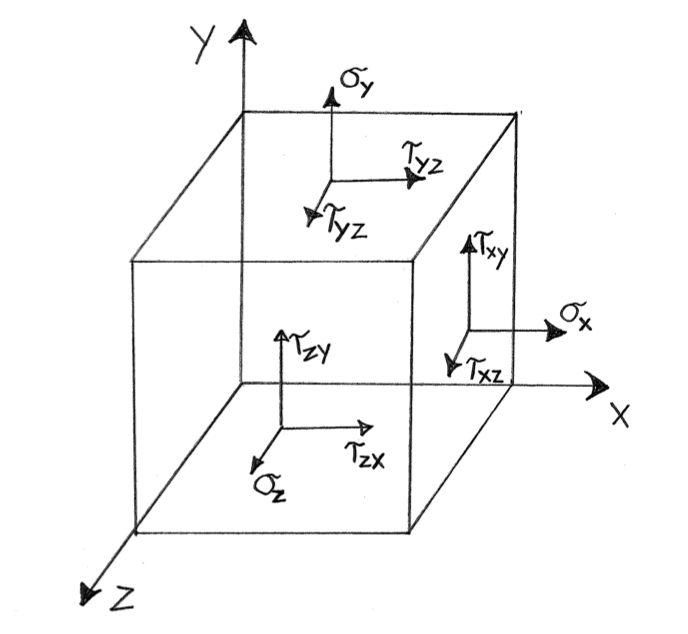
\includegraphics[width=8cm]{./images/physics_stress_box.png}
\caption{Stress in three dimensions.}
\label{fig:stress_box}
\end{figure}

The components of normal stress are denoted $\sigma_x$,
$\sigma_y$ and $\sigma_z$, one for each axial stress acting
perpendicular to a body face. Normal stress is either tension or
compression, often causing change in volume. Shearing stress is
denoted $\tau_{xy}$, $\tau_{yz}$ and $\tau_{zx}$, each
acting parallel or tangential to a body face causing it
to deform without particular volume change.
% Figure \vref{fig:stress-box} shows the notation used to define stress in three
% dimensions. The components of normal stress are denoted $\sigma_x$,
% $\sigma_y$ and $\sigma_z$, one for each axial stress.
% %
% Shear stress is denoted $\tau_{xy}$,
% $\tau_{yz}$ and $\tau_{zx}$. 
The first letter in the double subscript
indicates the \defit{plane} in which the stress acts, whereas the second
subscript indicates in which \defit{direction} the stress
acts.
%the coordinate direction which is normal to the plane in which the stress
%acts; the second subscript indicates the coordinate direction
%in which the stress acts. 
For example $\tau_{xy}$ has $x$ as its first
subscript therefore the stress acts in the $yz$-plane because the
direction $x$ is a normal to this plane. The second subscript
is $y$ indicting the actual stress direction.
%
We assume equilibrium of the element's volume, therefore $\tau_{xy}$
must be equal to $\tau_{yx}$ or else the element would not be at
rest. This means we only need three shear stress components since
$\tau_{xy} = \tau_{yx}$, $\tau_{yz} = \tau_{zy}$, and $\tau_{zx} =
\tau_{xz}$.
%Only three components of shear stress are
%needed, as only these three are independent ($\tau_{xy} = \tau_{yx}$,
%$\tau_{yz} = \tau_{zy}$ and $\tau_{zx} = \tau_{xz}$).
Altogether we only need the six independent quantities $\sigma_x$,
$\sigma_y$, $\sigma_z$, $\tau_{xy}$, $\tau_{yz}$ and $\tau_{zx}$ to completely
describe the state of stress at a given point in the
continuum \citebook{page~658}{book:fem-engineers}.
%
When considering stress in three dimensions we refer to the measure as
a force per volume, rather then the individual components as force per
area. The normal stress can be represented on vector form as
$\sigma = [ \sigma_{x}, \ \sigma_{y}, \ \sigma_{z} ]^T$ and the
sharing stress as 
$\tau = [ \tau_{xy}, \ \tau_{xz}, \ \tau_{yz} ]^T$.

\subsection{Strain Energy}
The potential energy stored within a deformed body is called \defit{strain
  energy}. Strain energy is calculated the same way, we calculate
work, but instead of relating force and displacement we use the stress
and strain induced in the body. The body's internal potential strain
energy is calculated as:

\begin{equation}
\label{eq:strain_energy}
E_S = 
\int_{V} \varepsilon \cdot \sigma \ dV +
\int_{V} \gamma \cdot \tau \ dV
\end{equation}

where the strain and stress vectors dotted and integrated over the
volume $V$ yields the internal potential strain energy. The integral
insures that the internal forces are distributed uniformly throughout
the volume \citebook{page~224}{book:applied_math}.
%
Because stress is a force per volume measure, the strain energy is
also a force per volume measure.

\subsection{Strain Energy Density}
The \defit{strain energy density} $dE_S$, is the strain energy
per unit volume, which can be obtained by
\citebook{page~625}{book:tim-mom}:

\begin{equation}
\label{eq:strain_energy_density}
dE_S = 
\int_0^\varepsilon \sigma \ d \varepsilon  +
\int_0^\gamma \tau \ d \gamma 
\end{equation}

and when stress-strain curves are introduced in section
\vref{sec:sscs}, this constitutes the area below such a curve. Strain
energy and strain energy density are directly related by the following
equation:

\begin{equation}
\label{eq:strain_energy_density_integral}
E_S = 
\int_V dE_S \ dV
\end{equation}

%\subsection{Strain energy density function}
%relates the strain energy density of a material to the deformation
%gradient.


% \subsection{Equilibrium for a Continuum}
% As described in section \vref{sec:principle-of-virtual-work},
% equilibrium for a continuum is defined in terms of the
% principle of virtual work. This principle states that: $\mbox{internal
%   virtual work} = -\mbox{external virtual work}$. To use this
% definition on a continuum we need to know how to calculate the
% internal and external virtual work. The internal virtual work for a
% continuum is defined as:

% \begin{equation}
% \label{eq:internal_virtual_work}
%   \mbox{internal virtual work:}
%   \int_{V} \delta \varepsilon \cdot \sigma \ dV +
%   \int_{V} \delta \gamma \cdot \tau \ dV
% \end{equation}

% where the transpose of the virtual normal strain vector $\varepsilon$ multiplied by
% the normal stress vector and integrated over the volume $V$ yields
% the internal virtual work. The integral insures that the internal
% forces are distributed uniformly throughout the volume
% \citebook{page~224}{book:applied_math}.

% The external virtual work is defined to be: $\mbox{virtual surface work} +
% \mbox{virtual body work}$. Forces acting upon the body (volume) are denoted
% $f_V$ and traction (surface forces) $f_S$, $\delta u$ is the virtual
% displacement vector, $V$ the volume and $S$ is the surface. The virtual
% work is calculated as described in section \vref{sec:virtual-work}
% and integrated over the volume and surface respectively:

% \begin{equation}
%   \mbox{virtual surface work:} \int_{S} \delta u \cdot f_S \ dS
%   \qquad
%   \mbox{virtual body work:} \int_{V} \delta u \cdot f_V \ dV 
% \end{equation}

% Substituting these definitions into the principle of
% virtual work, we obtain:

% \begin{equation}
%   \label{eq:povw}
%   \int_{V} \delta \varepsilon \cdot \sigma \ dV +
%   \int_{V} \delta \gamma \cdot \tau \ dV =
%   \int_{S} \delta u \cdot f_S \ dS +
%   \int_{V} \delta u \cdot f_V \ dV
% \end{equation}

% Consider equation \eqref{eq:povw}, when external forces are applied,
% the body reacts by either adjusting the virtual displacement or the
% level of stress.

\subsection{Equilibrium for a Continuum}
\label{sec:equilibrium-for-a-continuum}
As described in section \vref{sec:equilibrium-for-deobj}, equilibrium
for a deformable object is defined in terms of energy. Here we will
specify this definition for a continuum. Recall from section
\vref{sec:conser-of-me} that when an object has changed shape we
consider two states of the object and their energy relation. Equation
\eqref{eq:EW} is repeated below, it relates the
change in potential energy to the work done by kinetic
energy. Equilibrium for a continuum is precisely this, the relation
between the work done by external force, and the resulting internal
force measured as potential energy.

\begin{equation*}
- W = \Delta E_U
\end{equation*}

As normally done we set the initial potential energy $E_U^0 = 0$,
which means that the equation becomes: $- W = E_U^1$. The internal
potential energy is the strain energy for a continuum and is defined
in equation \eqref{eq:strain_energy} as:

\begin{equation*}
  E_S = \int_{V} \varepsilon \cdot \sigma \ dV +
  \int_{V} \gamma \cdot \tau \ dV
\end{equation*}

The work done by the external forces is defined to be:
$\mbox{surface work} + \mbox{body work}$.
Forces acting upon the body (volume) are denoted $f_V$ and traction
(surface forces) $f_S$, $u$ is the displacement vector, $V$ the volume
and $S$ is the surface. The work is calculated by integrating force times
displacement over the volume and surface, as described in section
\vref{sec:work}.

\begin{equation}
  \mbox{surface work:} \int_{S} u \cdot f_S \ dS
  \qquad
  \mbox{body work:} \int_{V} u \cdot f_V \ dV 
\end{equation}

A surface integral can be converted into a volume integral
using the Gauss divergence theorem. By doing this the total external
work can be expressed as
\citebook{page~49}{book:continuum-mechanics-mase}:

\begin{equation}
  \label{eq:external-work}
  \mbox{external work:}
  \int_{V} u \cdot f_V \ dV
\end{equation}

Substituting these definitions into the equation: $ -W= E_U^1$, we obtain:

\begin{equation}
  \label{eq:pompe}
  - ( \int_{V} u \cdot f_V \ dV ) =
  ( \int_{V} \varepsilon \cdot \sigma \ dV +
  \int_{V} \gamma \cdot \tau \ dV )
\end{equation}

Consider equation \eqref{eq:pompe}, when external forces are applied,
the body reacts by either adjusting the displacement or the level of
internal energy.

\section{Mechanical Properties}
\label{mechanical-properties}
We will now elaborate on how stress and strain is related. Mechanical
properties of a material describe how stress and 
strain are related in the given material.
%
As the stress and strain increases with the external force applied,
the material behaviour changes.
Mechanical properties are theoretically divided into different
phases based on how the material behaves. The first phase represents  
\defit{elastic deformation}, here the material absorbs the forces and
stores them as stress and strain. The second phase represents
\defit{plastic deformation}, during this phase the internal structures
of the material change permanently. If the amount of stress and
strain exceeds the point of \defit{fracture} the material will collapse.
Elastic deformation is reversible, but the other deformation types are not.
\citebook{page~344-345}{book:uni-physics}

% When a body is applied external force until it breaks, the material
% passes through different types for deformation. 

% In the first phase,
% denoted \defit{elastic deformation}, the material absorbs the forces and
% stores them as stress and strain. At some point the material is
% subjected to so much external force that it starts to break.
% In this second phase, termed \defit{plastic deformation}, the internal
% structure or property of the material changes. At some point the
% material cannot withstand anymore forces and it fractures. 

\subsection{Stress-strain Curves}
\label{sec:sscs}
To visualize how a material goes through the different
types of deformation, we look at stress-strain curves. A stress-strain
curve is a graph where measurements of stress as a function of
strain, are plotted. The graph should be interpreted as follows: When
moving away from origin along the $x$ axis, the material gets more and
more stretched (or compressed) depending on the direction. Normally
the stress-strain curve only includes stretch, which is positive along
the $x$ axis.
%
Isotopic materials yield the same stress-strain curve in
any direction, therefore only one stress-strain curve is needed. To
describe an anisotropic material more than one stress-strain curve is
needed.
%
The stress-strain curves in figure \vref{fig:stress-starin-overview},
show an overview of how to interpret the curves. Figure
\ref{fig:ssc-phaces} illustrates the different phases and figure
\ref{fig:ssc-points} the names of the transition points between the
phases. The transition point between linear and non-linear elasticity
is called \defit{proportional limit}. Between elastic and
plastic deformation it is called \defit{yield strength}, and the
material will break when reaching the \defit{fracture point}.
The maximum amount of stress during plastic deformation is called the
\defit{ultimate strength} limit.

\begin{figure}
  \centering
  \subfloat[Phases.]{
    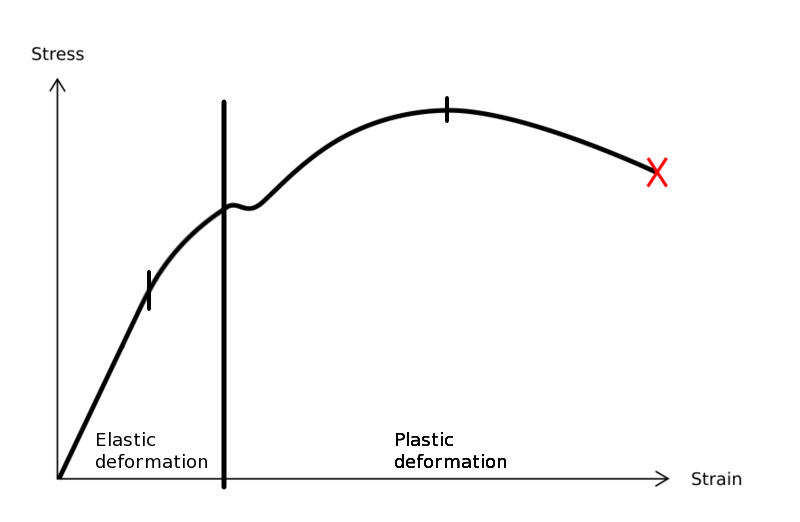
\includegraphics[width=7.5cm]{./images/physics_ssc_phases.png}
    \label{fig:ssc-phaces}
  }
  \subfloat[Points.]{
    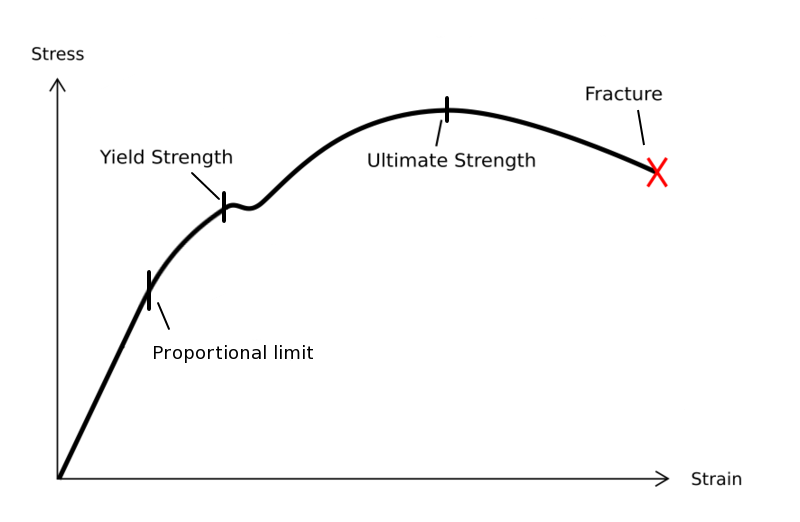
\includegraphics[width=7.5cm]{./images/physics_ssc_points.png}
    \label{fig:ssc-points}
  }
  \caption{Stress-strain curves overview.}
  \label{fig:stress-starin-overview}
\end{figure}

\subsection{Elastic Deformation}
\label{sec:elastic-deformation}
Elastic deformation or elasticity is the physical property of a
material when it deforms due to external forces applied, but returns to its
original shape when the forces are removed. The material returns to
the original form because the applied forces are stored as
stress and strain. The relation between stress and strain under
elastic deformation can be either linear, non-linear or both depending
on the material properties. \defit{Linear elasticity} is when strain
is directly proportional to stress. \defit{Non-linear elasticity} is
when the relationship between strain and stress is more complex and
can be approximated by a non-linear function. A material with both
properties is illustrated in figure \vref{fig:ssc-elasticity}.

\begin{figure}
  \centering
  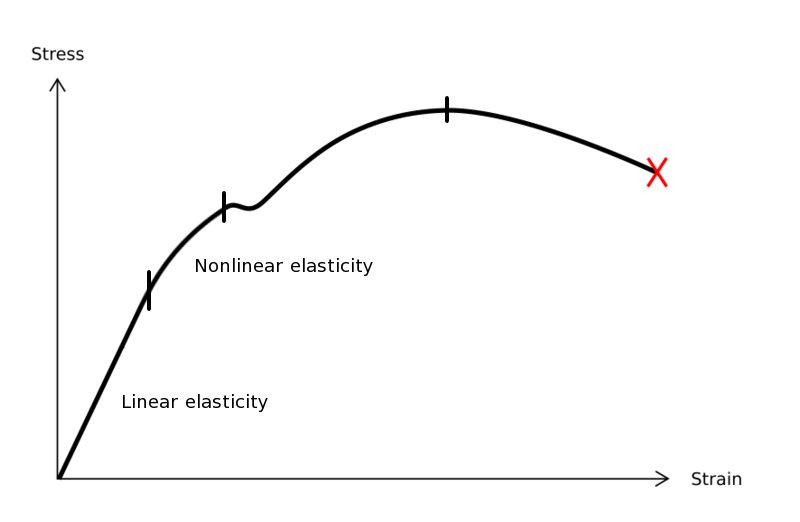
\includegraphics[width=7.5cm]{./images/physics_ssc_elasticity.png}
\caption{Stress-strain curve illustrating elastic deformation.}
\label{fig:ssc-elasticity}
\end{figure}

%Elastic deformation is instantaneous, which means that if we increase
%the strain we get an immediately change in stress.
Elastic deformation is
completely reversible. If the stress is reduced to its former value
the strain falls back to the original level
\citebook{page~183}{book:material-science}.

\subsection{Plastic Deformation}
\defit{Plastic deformation}, also known as \defit{plastic flow}, is an
irreversible deformation, which means that the body will not return to
its original configuration when the external forces are released. When
the amount of external forces exceeds the yield strength the plastic
deformation phase takes over.
%
Plastic deformation changes the rest shape of a material, by
changing its structure at the level of atoms. Atoms
are bound in a grid structure. This grid structure is
permanently changed by \defit{dislocations} along \defit{slip planes}.
\citebook{page~191-205}{book:material-science}.
%
An important property of plastic deformation is that it preserves the
volume of the material.
%
An example of a plastic deformable material is metal. If metal is
bent, the material's rest shape is permanently changed.
%
The stress-strain curve in figure \vref{fig:ssc-restshape} shows a
material that has gone through linear elastic deformation (stage 1-2),
non-linear elastic deformation (stage 2-3) and plastic deformation (3
and onwards). If at a point (4), the external forces are 
released, the material has obtained a permanent deformation and
therefore a new rest shape. The material returns to the new rest
shape via the dotted line.
%
If the material is, once more, subjected to external forces, the
deformation of the material follows the dotted line until the point of
yield strength is reached, and continues into plastic deformation if
enough forces are applied \citebook{page~159}{book:continuum-mechanics}.

\begin{figure}
  \centering
  \subfloat[Plastic deformation.]{
    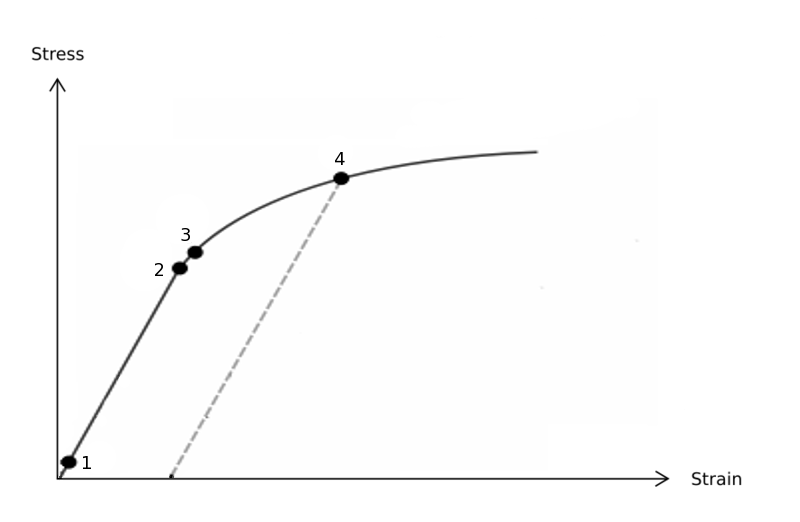
\includegraphics[width=7.5cm]{./images/physics_ssc_metal.png}
    \label{fig:ssc-restshape}
  }
  \subfloat[Stress-strain curve of strain hardening and necking.]{
    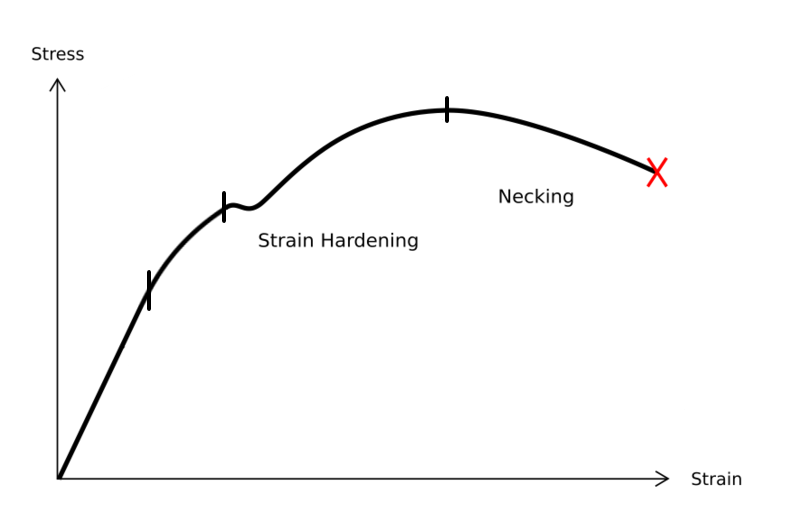
\includegraphics[width=7.5cm]{./images/physics_ssc_necking.png}
    \label{fig:ssc-necking}
  }
  \caption{Stress-strain curves illustrating plastic deformation.}
  \label{fig:ssc-plasticity}
\end{figure}

% \begin{figure}
%   \centering
% \end{figure}

Plastic deformation covers many distinct physical
processes. \defit{Strain hardening} and \defit{necking} are both
examples of physical processes which can be seen on the stress-strain
curve as illustrated in figure \vref{fig:ssc-necking}.
%
%\defit{Strain hardening}
Strain hardening or \defit{work hardening} is when a material becomes
increasingly saturated with dislocations. When more and more
dislocations are introduced the material starts to develop a
resistance against new dislocations. This resistance shows itself as a
strengthening of the material \citebook{page~194}{book:material-science}.
%
%\defit{Necking}
When a material is plastic deformed, and after the material's ultimate
strength limit has been reached \defit{necking} begins. The term
\defit{neck} refers to a point in the material where the material
gets weaker than the rest of the material. Necking is part of
the fracturing process for soft materials like metal
\citebook{page~223}{book:material-science}.

\subsection{Fracture}
If deformation exceeds the point of fracture, the material
collapses hereby releasing its internally stored forces. Material
collapse, known as fracture, is a subject of its own:
\defit{Fracture mechanics}. Fracture mechanics is elaborated in
section \vref{sec:fracture-mechanics}.

% \subsection{Additional Deformation Phenomena}

% \subsubsection{Fatigue}
% When a material is deformed in the elastic range, it completely returns to
% its original shape when forces are removed. But sometimes faults are
% introduced at the level of molecules. After many deformations,
% cracks will begin to appear, followed by fractures. The material will
% fracture with no apparent plastic deformation in between. 
% This phenomenon is known as \defit{fatigue}, and is most
% commonly observed in metals \citebook{page~225}{book:material-science}.

% \subsubsection{Hysteresis}
% Some elastic materials behave in one way when loaded, and another when
% unloaded. This phenomenon
% is know as hysteresis. Figure \vref{fig:ssc-hysteresis} is an example
% of a stress-strain curve for a material with hysteresis.
% %
% If the amount of work it takes to deform an object differs from
% the amount used to reverse the process, the material has
% hysteresis \citebook{page~345}{book:uni-physics}.

% \begin{figure}
%   \centering
%   \includegraphics[width=7.5cm]{./images/ssc-hysteresis.png}
% \caption{Stress-strain curve of hysteresis}
% \label{fig:ssc-hysteresis}
% \end{figure}

\subsection{Brittle and Ductile Materials}
\label{sec:brittle-ductile}
Solid materials can be categorised according to their material
properties. Before reaching the point of fracture, a material will
undergo plastic deformations to some extent.
%
If the amount of plastic deformation in a material is almost
non-existing, as in the case of glass, it is reasonable to neglect
this type of deformation. When this is the case the material is
considered \defit{brittle} and the point of yield strength $\approx$
fracture point.
%
Materials, like metal, where plastic deformation is important are
known as \defit{ductile} materials \citebook{page~345}{book:uni-physics}.
%
% Fatigue primarily occurs in ductile materials. Figure
% \vref{fig:ssc-brittle-and-ductile} illustrates stress-strain curves for
% typical brittle and a ductile materials.

% \begin{figure}
%   \centering
%   \subfloat[Brittle]{
%     \includegraphics[width=7cm]{./images/ssc-brittle.png}
%     \label{fig:ssc-brittle}
%   }
%   \subfloat[Ductile]{
%     \includegraphics[width=7cm]{./images/ssc-metal.png}
%     \label{fig:ssc-ductile}
%   }
%   \caption{Stress-strain curves for brittle and ductile materials}
%   \label{fig:ssc-brittle-and-ductile}
% \end{figure}


\subsection{Variations in the Material Properties}
Materials can have different properties when compressed compared
to when stretched. Concrete for example, is much stronger
when compressed than when stretched. Figure
\vref{fig:ssc-stretch-and-compression-fragture} illustrates this in one
stress-strain curve by using that compressive strain is negative. Here
the fracture point is much higher under compression that under
stretch.
%
The material can have a particular stress and strain relation under compression
and another when stretched, hereby yielding two different slopes, as
illustrated in figure \vref{fig:ssc-stretch-and-compression-moduli}.
% When this is the case we
%denote the elastic moduli $E_+$ and $E_-$. \\
%

\begin{figure}
  \centering
  \subfloat[Different fracture points.]{
    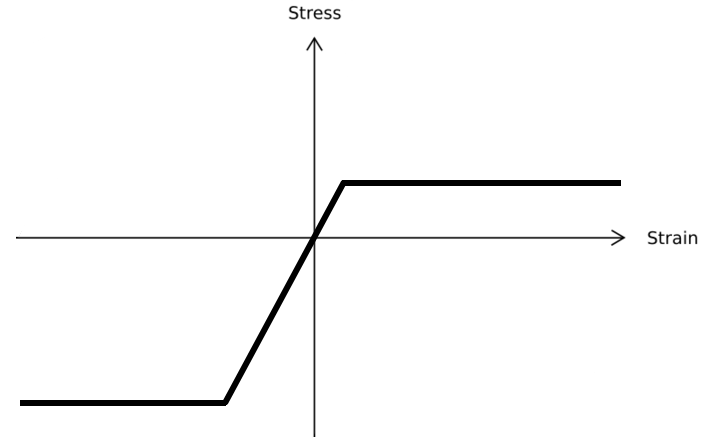
\includegraphics[width=7.5cm]{./images/physics_ssc_stretch_compression_fragture.png}
    \label{fig:ssc-stretch-and-compression-fragture}
  }
  \subfloat[Different slope.]{
    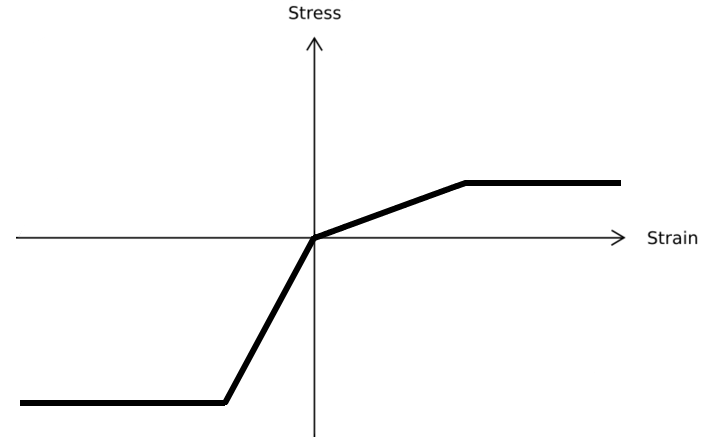
\includegraphics[width=7.5cm]{./images/physics_ssc_stretch_compression.png}
    \label{fig:ssc-stretch-and-compression-moduli}
  }
  \caption{Stress-strain curves of materials with different properties during compression contra stretch.}
  \label{fig:ssc-stretch-and-compression}
\end{figure}

% Material properties depend on many other parameters of the
% surroundings, like temperature, pressure and humidity.
% When modeling a material the influence of such phenomena most be
% taken into account individually.

% - Elasticity
% - - Material properties
\section{Linear Elasticity}
\label{sec:elasticity}
% material science, p. 181
% Because we want to model brittle material, only the elastic
% deformation of a material is of interest. Elastic deformation can
% either be linear, non-linear or both and the elastic properties depend
% on the material as described in section \vref{sec:elastic-deformation}.
% %
% In the following section we will introduce the linear elasticity
% theory for isotropic materials. 
% An \defit{isotropic material} is a material that has the same
% properties in all directions. 
%
When modeling brittle material, only the elastic
deformation of a material is of interest, and we shall assume that the
stress-strain relation is linear. Furthermore we shall assume that the
material is \defit{isotropic}, i.e. that it has the same properties is
all directions.
%
Linear elasticity in the simplest form is described by 
\defit{Hooke's law} of elasticity. Hooke's law relates deformation and
external forces by stating: \defit{Extension of a
material is in direct proportion with the forces acting upon it}. This is
true as long as the force does not exceed the elastic proportional
limit. The most commonly encountered form of Hooke's law is \defit{the
  spring equation}, which relates the force exerted by a spring to the
distance it is stretched or compressed by a spring constant $k$
measured in force per unit length ($N/m$). 

\begin{equation}
\label{eq:hooks_law}
    f = -k \cdot \Delta x
\end{equation}

The negative sign indicates that the force exerted by the spring is in
opposite direction of the displacement.
%
To extend Hooke's Law into three dimensions we need to introduce more
than one constant which relates forces and deformation. In keeping
with generally used terms in theory of linear elasticity these
constants are denoted moduli.
%
%Like the spring constant, a modulus relates forces to deformation hence
%stress to strain. A modulus relates stress and strain as follows:
%$\frac{stress}{strain}$.
%
More than one modulus enables us to relate the degrees of freedom in
three dimensions. There are many different moduli or constants in linear
elasticity but we only need two: the elastic modulus and Poisson's ratio,
and how they relate stress and strain to cover all degrees of freedom.

\subsection{Modulus of Elasticity}
The \defit{elastic modulus} or \defit{Young's modulus} $E$ relates normal
strain and normal stress and is defined to be:

\begin{equation}
\label{eq:normal_stress_over_normal_strain}
  E =  \frac{\mbox{normal stress}}{\mbox{normal strain}}
  = \frac{\sigma}{\varepsilon}
  \qquad \Leftrightarrow \qquad
  \varepsilon = \frac{\sigma}{E}
\end{equation}

The elastic modulus is
material dependent and can be found in reference books like
\citeabook{book:springer-materials}. Seen on a stress-strain curve a 
modulus is the slope of the linear piece of the graph. A high modulus 
indicates a hard or stiff material whereas a low modulus indicates a
soft elastic material.
%A relationship between $E$ and $G$ exists, this
%relationship includes elastic constant, referred to as Poisson's
%ratio. Poisson's ratio must be introduced before the relationship can
%be explained.

% below copied from tled report, spg tic om det er ham der har
% skrevet det
\subsection{Poisson's Ratio}
\label{sec:poissons_ratio}
When a body is stretched or compressed in one direction, it tends to
contract or expand in the opposite two directions. Poisson's ratio
$\nu$ is a direct measurement of this phenomenon for isotropic
materials. Consider a material in two dimensions, when it is
compressed by a force along the $x$-axis it results in the strain
$\varepsilon_x$. Due to the compression the material will expand 
$\varepsilon_y$ in the y direction, as follows:

\begin{equation}
  \varepsilon_y = - \nu \varepsilon_x
    \qquad \Leftrightarrow \qquad
    \nu =
    -\frac{\varepsilon_x}{\varepsilon_y} =
    -\frac{\Delta x / x}{\Delta y / y}
\end{equation}

Here $\nu$ is Poisson's ratio, relating the compression and
expansion. To express this as stress, we use equation
\eqref{eq:normal_stress_over_normal_strain} and get:

\begin{equation}
  \varepsilon_y = - \nu \varepsilon_x = - \nu \frac{\sigma_x}{E}
\end{equation}

Like the elastic modulus, Poisson's ratio can be found in reference
books.

\subsection{Relating Stress and Strain in Three Dimensions}
\label{sec:stress-strain-relation-in-3d}
To relate stress and strain in three dimensions, we need to combine
the elastic modulus and Poisson's ratio in all dimensions.
%
%If stress other than pure tensile or pure shearing is applied, the
%material behaviour gets a bit more complicated. 
%
Consider a cubic element with normal stress $\sigma_x$, $\sigma_y$
and $\sigma_z$ acting in the $x$, $y$, and $z$ direction, respectively.
%
% According to equation 
% \eqref{eq:normal_stress_over_normal_strain} the cube will stretch in the
% x direction by a strain $\varepsilon_x = \sigma_x / E$, and contract
% by a tensile strain of $-\nu \sigma_x / E\ $ in
% the other two directions due to the effect described by Poisson's ratio. 
% Similarly the reaction to tensile stress $\sigma_y$ in the y
% direction will be a tensile strain of $-\nu \sigma_y / E\ $ in
% the x and z direction. 
% % If a stress is applied which is not purely tensile or purely shear
% % then the behavior of the material is more complicated. When a object is
% % subjected to external forces then, as a direct
% % conseqiense of posion's ratio, if one direction is stretched, then
% % others will compress. 
% When modeling isotropic materials, this
% relationship will be uniformly distributed between the other directions
% \citebook{page~185-187}{book:material-science}. \\
% %
%
% From Hooke's Law and Poisson's ratio we obtain an expression of
% tensile strain in each direction:
%
% %It is possible to generalize Hooke's Law into three dimensions
% %via Poisson's ratio, and make all directions dependent:
%
Due to the stress component, $\sigma_x$, the cube will stretch (if
$\sigma_x > 0$) in the $x$ direction by the amount which according to
equation \eqref{eq:normal_stress_over_normal_strain} is $\varepsilon_x
= \sigma_x / E$ and contract in the $y$- and $z$-direction by an amount of
$-\nu \sigma_x /E$. Similarly for the remaining two stress
components. The total deformation of the cube is now found by adding
the various contributions \citebook{page~187}{book:material-science}:

\begin{equation}
\label{eq:hookes-law-in-3d}
\begin{aligned}
    \varepsilon_x &= \frac {1}{E} \left [ \sigma_x - \nu \left (
        \sigma_y + \sigma_z \right ) \right ] \\
    \varepsilon_y &= \frac {1}{E} \left [ \sigma_y - \nu \left (
        \sigma_x + \sigma_z \right ) \right ] \\
    \varepsilon_z &= \frac {1}{E} \left [ \sigma_z - \nu \left (
        \sigma_x + \sigma_y \right ) \right ]  
\end{aligned}
\end{equation}

In equation \eqref{eq:hookes-law-in-3d} the relation between normal
stress and strain are completely defined by the two constants $E$ and
$\nu$. These constants can also be used to relate shearing stress and
strain.
%
%Note that this only accounts for stress and strain in the normal
%directions. As we also model shearing stress and strain, these
%quantities most also be taken into account.
%
The relationship between shearing stress and shearing strain is 
called the \defit{Shear modulus} or \defit{modulus of rigidity} and is
denoted $G$.

\begin{equation}
\label{eq:shearing_stress_over_shearing_strain}
  G 
  %= \mu
  = \frac{\mbox{shear stress}}{\mbox{shear strain}}
  = \frac{\tau_{xy}}{\gamma_{xy}}
  \qquad \Leftrightarrow \qquad
  \gamma_{xy} = \frac{\tau_{xy}}{G}
\end{equation}

The shear modulus can be deduced from $E$ and $\nu$ as done in
\citebook{page~9-10}{book:theory-of-elasticity}, the relation is:

\begin{equation}
\label{eq:EG-relation}
  G = \frac{E}{2(\nu+1)}
\end{equation}

Shearing in one direction does not affect shear in other
directions. Note that shear is independent of normal stress and
strain \citebook{page~266}{book:deformable-solids}. For shear in three
dimensions, the equations are defined as:

\begin{equation}
\label{eq:3d-shear-ss-relation}
  \gamma_{xy} = \tau_{xy} / G
  \qquad
  \gamma_{yz} = \tau_{yz} / G
  \qquad
  \gamma_{zx} = \tau_{zx} / G
\end{equation}


% Fracture Mechanics
\section{Fracture Mechanics}
\label{sec:fracture-mechanics}
\defit{Fracture mechanics} describes what happens to a material when
the fracture point limit has been exceeded.
%
When the material reaches this limit, a fracture is initiated at a
specific \defit{crack point} within the material. The fracture
propagates by opening a crack inside the material along a
\defit{fracture plane}. The crack can be described by connected
\defit{crack surfaces}. The crack opens to release
potential energy accumulated within the material. The internal potential
strain energy, is used to create
new \defit{crack surfaces} by ripping part of the body into surfaces.
This conversion of body to surface requires work, which is
how the energy is released \citebook{page~218}{book:material-science}.
%
The \defit{crack length} is determined by the amount of internally
stored energy contra how much energy it takes to create the new surfaces.
%
When considering an isotopic material in three dimensions, we idealize
the crack surfaces by using two surfaces, which form a lens as
illustrated in figure \vref{fig:crack-surfaces}.

% \begin{figure}
%   \centering
%   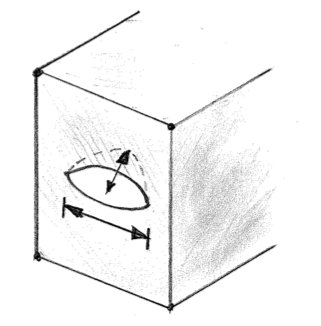
\includegraphics[width=6cm]{./images/physics_crack_surfaces_0.png}
%   \caption{Crack surfaces.}
%   \label{fig:crack-surfaces}
% \End{figure}

\begin{figure}
  \begin{minipage}[b]{0.5\linewidth}
    \centering
    \subfloat[Half lens.]{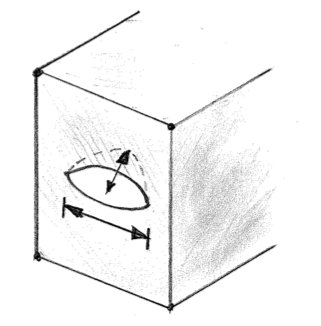
\includegraphics[width=70mm]{./images/physics_crack_surfaces_0.png}}
  \end{minipage}
  \hspace{0.5cm}
  \begin{minipage}[b]{0.5\linewidth}
    \centering
    \subfloat[Quarter of a lens.]{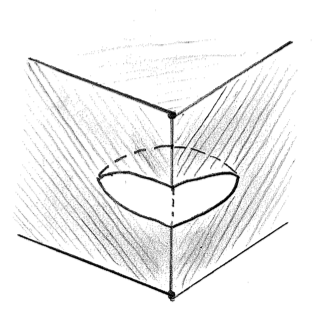
\includegraphics[width=70mm]{./images/physics_crack_surfaces_1.png}}
  \end{minipage}
  \caption{Two crack surfaces forming a lens.}
  \label{fig:crack-surfaces}
\end{figure}

%The analytical formulas for calculating the strain energy along the
%crack in three dimensions are very complex and beyond the scope of 
%will be omitted, but
%We will return to the subject of fracture mechanics when constructing
%a discrete model in section \vref{sec:discrete-fracture-mechanics}.

% crack initial via max pr stress.
\subsection{Crack Initialization}
\label{sec:physics_crack_init}
% include that there are teories for having more than one crack init.
There are different theories of how to calculate the crack
initialization point. We use: \defit{maximum principal stress} since this
technique has proved suitable for brittle materials
\citebook{page~370}{book:strength-materials}.
%
\defit{Principal stress} is a measure where both shearing and normal
stress is incorporated, yielding three vectors. The longest vector of
the three reveals in which direction the maximum stress points in a
given point within the material. The method of maximum principal finds
the maximum principal stress of all points in the material, yielding
the precise point and direction of the stress.
%
If this stress exceeds the fracture point ($\sigma_F$), the material
breaks in this precise location. If a material has different
fracture point limits when stretched or compressed, they are
denoted: $\sigma_F^+$ and $\sigma_F^-$.
% 
How to calculate the principal stress based on normal and shearing
stress will be elaborated in section
\vref{sec:principal_values_and_directions}, when linear transformation
has been introduced.
%
The principal stress also contains information about how the crack
surfaces will form. The vector direction defines the normal of the
crack plane.

\subsection{Crack length}
The energy it takes to form the new surface is determined by the
crack surfaces area and the \defit{strain energy release rate}, which
is a material property.
The length of the crack is determined by the amount of strain energy
stored in the point where the crack opens and the amount it takes to
create the crack surfaces. The amount of energy used to create a
surface in a given material depends upon the material itself and on
the area of the crack surfaces. The area of the surfaces when using
the lens form is further approximated by using a circle. This is done
because the lens is much wider that thick and therefore a circle
covers most of the area as illustrated in figure
\vref{fig:crack-surfaces-from-above}, where the crack is seen from
above. The circle area is calculated by: $A = \pi a^2$.

% \begin{figure}
%   \centering
%   \includegraphics[width=6cm]{./images/material-science-p218-f9-31.png}
%   \caption{Crack surfaces seen from above}
%   \label{fig:crack-surfaces-from-above}
% \end{figure}

\begin{figure}
  \centering
  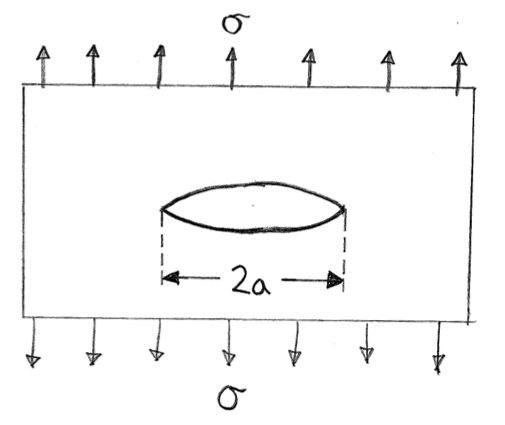
\includegraphics[width=7cm]{./images/physics_crack_surfaces_from_above.png}
  \caption{Crack surfaces seen from above.}
  \label{fig:crack-surfaces-from-above}
\end{figure}


%And can be use to calculate the stress at the \defit{crack tip}. The
%stress $\sigma_{tip}$ for an elliptical section is given by
%\citebook{page~218}{book:material-science}:

%\begin{equation}
%\sigma_{tip} = 2 \sigma \left( \frac{a}{\rho} \right)^{1/2}
%\end{equation}

%Where $\rho$ is the radius for the \defit{dominant zone}. The dominant
%zone ...

% *** insert figure from: applied solid mechanics, section 9.3.2


%The strain energy is calculated as:
%\begin{equation}
%  E_E = \int_V \sigma \cdot \varepsilon
%\end{equation}

%But for at crack of unit width, can be approximated by:
%\begin{equation}
%  E_E = \sigma \varepsilon V
%  = \frac{\sigma^2 V}{E}
%  = \frac{\sigma^2 \pi a^2}{E}
%\end{equation}

%\begin{equation}
%  U_S = = 2 G_C a = 4 \gamma a
%\end{equation}

%We use the energy relation from  \vref{sec:energy-} to relate the 

%\begin{equation}
%  U = U_E + U_S = 0 \Leftrightarrow - U_E = U_s
%\end{equation}

%Energy release:

The crack continues to grow until the strain energy cannot expand 
the crack surfaces further. Figure \vref{fig:energy-release-graph}
illustrates an example of this.
%
The graph $E_C$ depicts the amount of energy it takes to produce the
crack surfaces as a function of the crack length $a$. 
%
%This means that larger crack surfaces requires more energy to produce.
%
The graph $E_S$ is the internal strain energy in the body.
%
Focusing on graph $E_T$ this graph describes the total
energy ($E_T = E_C + E_S$), here the fracture point is reached
at the dotted line, and a crack is initialized, hereby releasing
energy.
%
Looking at the strain energy function $E_S$ we see that this energy
rapidly increases as the crack starts to propagate.
%
When the $E_T$ graph crosses the $x$ axis, there is no more energy
left and the crack propagation stops.

\begin{figure}
  \centering
  \subfloat[Strain contra surface energy.]{
   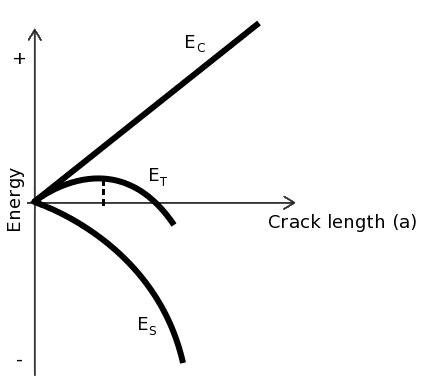
\includegraphics[width=6cm]{./images/physics_energy_release_graph.png}
   \label{fig:energy-release-graph}
  }
  \qquad
  \subfloat[Derivatives of strain and surface energy.]{
   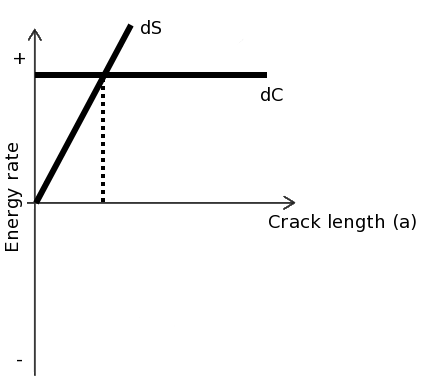
\includegraphics[width=6cm]{./images/physics_energy_graph.png}
   \label{fig:energy-graph}
  }
  \caption{Strain contra surface creation energy.}
  \label{fig:energy-graphs}
\end{figure}

Figure \vref{fig:energy-graph} illustrates the energy derivatives of
$E_C$ and $E_S$ from figure \vref{fig:energy-release-graph}. Here the
point where the strain energy exceeds the surface creation energy
becomes directly apparent \citebook{page~219-221}{book:material-science}.
%
In figure \vref{fig:energy-graph}, the following notation is used:

\begin{equation*}
dS = \frac{\partial E_S}{\partial a} \qquad \qquad dC = \frac{\partial E_C}{\partial a}
\end{equation*}



% open via energy, 
%\subsection{Energy}

% below copied from wiki:
% http://en.wikipedia.org/wiki/Strain_energy_release_rate
%Strain energy release rate (or energy release rate) is the energy
%dissipated during fracture per unit of newly created fracture surface
%area
% above copied from wiki: 
% http://en.wikipedia.org/wiki/Strain_energy_release_rate

\subsection{Crack propagation}
%For the crack to reach the materials outer surfaces, the crack must
%propagate all the way to this surface. 
%
% korteste vej til overfladen.
%The crack always steers towards the outer surface, hereby releasing
%the maximum amount of energy possible \citebook{}{}.
%
% ref som siger at hvis der allerede er en crack, forsættes denne.
%
Brittle material often has a single crack propagating through the
entire material \citebook{section~9.1}{book:solid-mechanics}.
%
% hastighed: lydens.
Once the crack begin to propagate, the stress required for further
propagation decreases as $a$ increases and therefore the crack
accelerates rapidly \citebook{page~220}{book:material-science}.

% note på at det med vinkler er realistisk for hårde materialer.



% energi ophobes
% når energien når over det niveau hvor sigma_max difinere arealet A
% laves de nye surfaces, og alt energien frigives.




% \subsection{Generalized stress modes}
% When the crack propagated it can be stressed by deformation
% of the body.
% This kind of stress is generalized into three different modes. Normal
% stress ... to \defit{opening mode} or \defit{mode I}, where the crack
% surfaces are perpendicular to the crack plane. In plane-shear result in \defit{sliding mode} or
% \defit{mode II}, here the displacement of the crack surfaces is in the
% plane of the crack and perpendicular to the crack front. The last,
% \defit{mode III} or \defit{tearing mode} is caused by out of plane
% shear \citebook{page~9}{book:elementary-fm}. The three modes are
% illustrated in figure \vref{}. Often more than one mode is
% pressent at the same time, when this happens we call it \defit{mixed
%   mode}.

% \begin{figure}
%   \centering
%   \includegraphics[width=5cm]{./images/elementary-fm-p25-f2-1.png}
%   \caption{The three modes of stress in the crack front}
%   \label{fig:stress-in-crack-front}
% \end{figure}
